\documentclass[12pt,a4paper,oneside]{book}
\usepackage[left=2cm,right=2cm,top=2cm,bottom=2cm]{geometry}
\usepackage[utf8]{inputenc}
\usepackage[T1]{fontenc}
\usepackage{amsmath,amsfonts,amssymb}
\usepackage{graphicx}
\usepackage[french]{babel}
\usepackage{listings} % pour insérer du code source
\usepackage{lmodern}
\usepackage{hyperref}
\usepackage{fancyhdr}
\usepackage{graphicx}
\usepackage{eso-pic} % nécessaire pour mettre des images en arrière plan
\usepackage{array}	
\usepackage{fancyhdr} % pour les en-têtes et pieds de pages
\usepackage{fancybox}
\usepackage{hyperref}
\usepackage{layout}
\usepackage{color}
\usepackage{tikz}
\usepackage{pifont}
\usepackage{titlesec}
\usepackage{color}
\usepackage{rotating}
%\usepackage[style=numeric]{biblatex}
\usepackage[Glenn]{fncychap} % pour customiser le style du titre \chapter
\usepackage{type1cm} % aussi pour les lettrines
\usepackage{lettrine}
\usepackage{longtable}
\usetikzlibrary{calc}
\usetikzlibrary{decorations.pathmorphing}
\usepackage{array,multirow,makecell}
\usepackage{setspace}
\usepackage{wrapfig}
\usepackage{sidecap}
\onehalfspacing % pour l'interligne
\setcellgapes{1pt}
\usepackage{array}
\usepackage{minipage-marginpar}
\usepackage{shorttoc} % Pour creer plusieurs tables de matieres
\makegapedcells
\newcolumntype{R}[1]{>{\raggedleft\arraybackslash }b{#1}}
\newcolumntype{L}[1]{>{\raggedright\arraybackslash }b{#1}}
\newcolumntype{C}[1]{>{\centering\arraybackslash }b{#1}}
\newcolumntype{M}[1]{>{\centering\arraybackslash}m{#1}}


%customization des \textbullet
\newcommand*{\tikzbullet}[2]{%
  \setbox0=\hbox{\strut}%
  \begin{tikzpicture}
    \useasboundingbox (-.25em,0) rectangle (.25em,\ht0);
    \filldraw[draw=#1,fill=#2] (0,0.5\ht0) circle[radius=.45em];
  \end{tikzpicture}%
}




%%%%%%%%%%%%%%%%%%%style front%%%%%%%%%%%%%%%%%%%%%%%%%%%%%%%%%%%%%%%%% 
\fancypagestyle{front}{%
        \fancyhf{}%on vide l'en-tête
        \fancyfoot[C]{\thepage}
        \renewcommand{\headrulewidth}{0pt}%trait horizontal pour l'en-tête
        \renewcommand{\footrulewidth}{1pt}%trait horizontal pour le pied de page
        }
                
                
                
                
                
                
                
                
%%%%%%%%%%%%%%%%%%%style main%%%%%%%%%%%%%%%%%%%%%%%%%%%%%%%%%%%%


\newcommand{\chaptertoc}[1]{\chapter*{#1}
\markboth{\slshape\MakeUppercase{#1}}{\slshape\MakeUppercase{#1}}}

        \fancypagestyle{main}{%
                \fancyhf{}
                \renewcommand{\chaptermark}[1]{\markboth{\chaptername\ \thechapter.\ ##1}{}} % redéfinition pour avoir ici les titres des chapitres des sections en minuscules
                
                
                \pagestyle{fancy}
                \renewcommand\headrulewidth{1pt}
                \fancyhead[C]{titre du theme}
                
                
                \fancyfoot[L]{\textbf{Mémoire rédigé et soutenu par xxxxxxxxxxxx}}
                \fancyfoot[R]{\thepage}%
                \renewcommand{\headrulewidth}{1pt}%trait horizontal pour l'en-tête
                \renewcommand{\footrulewidth}{1pt}%trait horizontal pour le pied de page
                }
            
            
            
            
            
            
            
            
            
            
%%%%%%%%%%%%%%%%%%%style pied%%%%%%%%%%%%%%%%%%%%%%%%%%%%%%%%%%%%%%%%%  
        \fancypagestyle{back}{%
                \fancyhf{}%on vide l'en-tête
                \fancyfoot[L]{\textbf{Mémoire rédigé et soutenu par xxxxxxxxxxxxx}}
                \fancyfoot[R]{\thepage}%
                \renewcommand{\headrulewidth}{0pt}%trait horizontal pour l'en-tête
                \renewcommand{\footrulewidth}{1pt}%trait horizontal pour le pied de pages
                }
                
                
                
                
                
                
%%%%%%%%%%%%%%%%%%% Définition des couleurs %%%%%%%%%%%%%%%%%%%
\definecolor{green1}{HTML}{556627}
\definecolor{green2}{HTML}{B7CA79}
\definecolor{green3}{HTML}{8FCF3C}
\definecolor{green4}{HTML}{1D702D}
\definecolor{green5}{HTML}{456B35}


\definecolor{blue1}{HTML}{1370e9}
\definecolor{blue2}{HTML}{2da9e9}










\begin{document}


\frontmatter %Entete du document
\pagestyle{front} %style des en-têtes pour cette portion

\chapter{Dédicace}
\paragraph{}
\paragraph{}
\paragraph{}
\begin{flushright}
 Je dédie ce mémoire a toute ma famille.
\end{flushright}
 





\chapter*{Remerciements}         % ne pas numéroter
\phantomsection\addcontentsline{toc}{chapter}{Remerciements} % inclure dans TdM

Texte des remerciements en prose.



\shorttableofcontents{Sommaire}{1}
\addcontentsline{toc}{chapter}{Sommaire}


\chapter{Abréviations}




\renewcommand{\listfigurename}{Liste des figures}
\listoffigures
\addcontentsline{toc}{chapter}{Liste des figures}


\listoftables
\addcontentsline{toc}{chapter}{Liste des tableaux}


\chapter*{Résumé}                      % ne pas numéroter
\phantomsection\addcontentsline{toc}{chapter}{Résumé} % inclure dans TdM

\begin{otherlanguage*}{french}
  Texte du résumé en français.
\end{otherlanguage*}

\chapter{Abstract}

\paragraph{}
The Startup INSBI (Institute Business Intelligence) is a newly created company which in its offer has a list of service that revolves around solutions of digitalization of companies and business intelligence. In order to make a name for itself in the market INSBI has produced and launched its first product which is Hosteline. Hosteline is an online hospitality platform that targets hotel owners and places their premises at the disposal of customers who in turn can book these different premises. Hosteline is a web portal that brings together hotels and provides comparative access to customers of this platform. Through this platform, hotel customers will have advantages both in terms of prices and the facilities that these hotels can offer thanks to its loyalty program. This system when put into production will generate a large amount of data through its transactional system. Knowing how useful these data are but not enough in the raw state, the INSBI management wants to set up a decision-making system to be able to exploit this data and to draw the strategic choices and decisions to make the product grow offering a better quality of service to its consumers. These is where we came into the game to set up a Reporting system that will serve data from operational systems in readable and easily interpretable formats. Our job was to give satisfaction to a specific need recorded in a specifications book with well-defined cost and time constraints. In this thesis we will highlight, the working method, the evolution of the work at INSBI and the follow-up that was ours throughout the duration of our internship. Thanks to this project we could put into practice lessons learned during our training and it permitted us to learn more about business intelligence and many other new concepts.

















	
\mainmatter
\pagestyle{main}

\chapter*{Introduction}
\addcontentsline{toc}{chapter}{Introduction}

\paragraph{}
L’avènement des TIC (Technologies de l’information) vient changer notre façon de vivre en la rendent plus simple. Le secteur hôtelier n’est pas exclu de ces changements et proposer ses services sur internet n’est plus un lux mais un besoin fondamentale pour toute entreprise hôtelière qui souhaite rester compétitive. Sur la toile les sites web d’hôtels se multiplient et tout particulier ou entreprise cherchent un ou plusieurs locaux en ligne à une large gamme de site web d’hôtels à sa portée. Le problème quand les possibilités sont large et non exhaustives est que on n’a pas toujours le temps de visiter ces plateformes une par une et comparer leurs offres selon nos préférences. Des plateformes telles que Booking.com, Accordhotel.com et autres offrent une solution qui répond a ce problème de comparaison de prix et d’offres toujours est-il que le contexte et les particularités camerounaises et Africaines n’est pas toujours retrouvée. En effet sur les plateformes de ce type on retrouve des hôtels conventionnels qui respectent certaines normes et standards occidentaux. A titre d’exemple le ministère du tourisme reconnais officiellement 250 hôtels accrédité au Cameroun ce qui ne représente pas 30\% du nombre réel d’établissements hôtelier du pays. Parmi les hébergeurs laissés on retrouve les propriétaires d’auberges, certaines résidences hôtelières, Appartements meublé, Villa et plein d’autre encore. Hosteline s’inspire des plateformes citées plus haut en adaptant le concept au milieu et aux coutumes Camerounaises. En effet Hosteline est une plateforme ouvert à tout type d’hébergeurs et hôteliers qui souhaitent se mettre à la disposition des clients et potentiels clients par le web.
	\paragraph{}
	Lorsque la plateforme sera lancé et tournera à plein régime la quantité de données cumulé sur une année sera énorme et en exploitant la plateforme sur plusieurs année encore ne produira qu’une masse de données conséquente. Pour anticiper sur les besoins de s’informer grâce à ces données  qui iront grandissant, Mr Kendjio le fondateur de Hosteline souhaite se munir d’un système décisionnel pour être prêt à exploiter et tirer avantage de ce volume important de données. La mise en œuvre de ce système décisionnel est le but de la rédaction du présent mémoire. Ce mémoire est organisé en deux parties majeures.\\
Dans la partie une, nous présentons les concepts de base du Business Intelligence dans le chapitre un. Dans le chapitre deux nous parlons des systèmes de gestion hôtelières en générale et de Hosteline en particulier.\\
	Dans la deuxième partie, le chapitre trois donnes les détails sur le cahier des charges. Dans les chapitre quatre, cinq et six nous présentons les méthodes d’analyse, de conception  puis le déploiement de de la solution respectivement.




\part{ÉTAT DE L'ART}

\chapter{Synthèse Bibliographique}

\section{Business Intelligence}
	\subsection{Introduction}
  		\paragraph{}
  		Dans le monde les grandes entreprises dans leurs activités journalières produisent une quantité importante de données qui a long terme devient en quantité astronomiques. Le besoin d’exploiter ces données a des fin de pilotage des entreprises a fait naitre le Business Intelligence encore appelé Intelligence Economique ou encore Informatique décisionnel qui permet d’étudier l’environnement de l’entreprise aux moyens des données qu’elle possède. Les données étant en grande quantité, il faut le nettoyer, les structures avant de les stocker dans ce qu’on a appelé Data Warehouse (Entrepôt de données en français).
  
  		\paragraph{}
  Le concept de Data Warehouse, tel que connu aujourd’hui, est apparu pour la première  fois en 1980 ; l’idée consistait alors à réaliser une base de données destinée exclusivement au processus décisionnel. Les nouveaux besoins de l’entreprise, les quantités importantes de données produites par les systèmes opérationnels et l’apparition des technologies aptes à sa mise en œuvre ont contribué à l’apparition du concept « Data Warehouse » comme support aux systèmes décisionnels.
  
  
	\subsection{Les systèmes décisionnels}
  		\paragraph{}
  L’entrepôt de données est au centre du système décisionnel et sa raison d’être est la mise en place de ces systèmes décisionnels. Nous allons ici rappeler quelques définitions qui serviront ont mieux expliqué la suite.
  \paragraph{}
  Selon Jean-Louis Le Moigne,  « Le système d’information est l’ensemble des méthodes et moyens de recueil de contrôle et de distribution des informations nécessaires à l’exercice de l’activité en tout point de l’organisation. Il a pour fonction de produire et de mémoriser les informations, de l’activité du système opérant (système opérationnel), puis de les mettre à disposition du système de décision (système de pilotage) » [Le Moigne 1977].
  \paragraph{}
  Selon Wikipédia, « L’informatique décisionnelle est l'informatique à l'usage des décideurs et des dirigeants    d'entreprises ».
  \paragraph{}
  De ces définition on retient que le système opérationnel et le système décisionnel sont des parties du                  système d’information. 
 


\begin{center}
	\begin{longtable}{|p{0.15\textwidth}|p{0.35\textwidth}|p{0.4\textwidth}|}
		\caption{Résume des différences entre le Transactionel et décisionnel.} 
		\label{Transactionel vs descisionel}
		\\
		
		
		\hline 
		\textbf{Critere} & 
		\textbf{Transact} &
		\textbf{discisionel}
		\\
		
		
		\endfirsthead
		\caption[]{Résume des différences entre le Transactionel et décisionnel (suite)} 
		\\
		\hline 
		\textbf{Différence} & 
		\textbf{Transactionel} &
		\textbf{déscisionel}
		\\
		\hline
		\endhead
		\hline
		\endfoot
		\hline
		
		
		\hline
		par les données &  
		
		\begin{description}
		 \item Orienté applications
		 \item Situation instantanée
		 \item Donnée détaillées et codées non redondantes
		 \item Données changeantes constamment
		 \end{description} &
		 
		 \begin{description}
		 \item Orienté thèmes et sujets
		 \item Situation historique
		 \item Informations agrégées cohérentes souvent avec redondance
		 \item Informations stables et synchronisées dans le temps
		 \end{description}
		\\ 
		
		\hline
		L’usage &  
		\begin{description}
		 \item Assure l’activité au quotidien
		 \item Pour les opérationnels
		 \item Mises à jour et requêtes simples
		 \item Temps de réponse immédiats
		 \end{description} &
		\begin{description}
		 \item Permet l’analyse et la prise de décision
		 \item Pour les décideurs
		 \item Lecture unique et requêtes complexes transparentes
		 \item Temps de réponse moins critiques
		 \end{description}
		\\  
		
		\hline 
	\end{longtable} 
\end{center}

\paragraph{}
	Ces différences font ressortir la nécessité de mettre en place un système répondant aux besoins décisionnels. Ce système n’est rien d’autre que le « Data Warehouse ».


\section{Le Data Warehouse}
 \subsection{Définition}
 Bill Inmon définit le Data Warehouse, dans son livre considéré comme étant la référence dans le domaine ``Building the Data Warehouse'' [Inmon, 2002] comme suit:
 
« Le Data Warehouse est une collection de données orientées sujet, intégrées, non volatiles et évolutives dans le temps, organisées pour le support d’un processus d’aide à la décision. »

Les paragraphes suivants illustrent les caractéristiques citées dans la définition d’Inmon.\\
\textbf{Orienté sujet}: le Data Warehouse est organisé autour des sujets majeurs de l’entreprise, contrairement à l’approche transactionnelle utilisée dans les systèmes opérationnels, qui sont conçus autour d’applications et de fonctions telles que : cartes bancaires, solvabilité client…, les Data Warehouse sont organisés autour de sujets majeurs de l’entreprise tels que : clientèle, ventes, produits…. Cette organisation affecte forcément la conception et l’implémentation des données contenues dans le Data Warehouse. Le contenu en données et en relations entre elles diffère aussi. Dans un système opérationnel, les données sont essentiellement destinées à satisfaire un processus fonctionnel et obéit à des règles de gestion, alors que celles d’un Data Warehouse sont destinées à un processus analytique.\\
\textbf{Intégrée }: le Data Warehouse va intégrer des données en provenance de différentes sources. Cela nécessite la gestion de toute incohérence.\\
\textbf{Evolutives dans le temps} : Dans un système décisionnel il est important de conserver les différentes valeurs d’une donnée, cela permet les comparaisons et le suivi de l’évolution des valeurs dans le temps, alors que dans un système opérationnel la valeur d’une donnée est simplement mise à jour. Dans un Data Warehouse chaque valeur est associée à un moment
« Every key structure in the data warehouse contains - implicitly or explicitly -an element of time » [Inmon, 2000].\\
\textbf{Non volatiles} : c’est ce qui est, en quelque sorte la conséquence de l’historisation décrite précédemment. Une donnée dans un environnement opérationnel peut être mise à jour ou supprimée, de telles opérations n’existent pas dans un environnement Data Warehouse. Organisées pour le support d’un processus d’aide à la décision : Les données du Data Warehouse sont organisées de manière à permettre l’exécution des processus d’aide à la décision (Reporting, Data Mining…).

 \subsection{Historique}
 	L’origine du concept « Data Warehouse » D.W (entrepôt de données en français) remonte aux années 80, durant lesquelles un intérêt croissant au système décisionnel a vu le jour, dû essentiellement à l’émergence des SGBD relationnel et la simplicité du modèle relationnel et la puissance offerte par le langage SQL, au début, le Data Warehouse n’était rien d’autre qu’une copie des données du système opérationnel prise de façon périodique, dédiée à un environnement de support à la prise de décision. Ainsi, les données étaient extraites du système opérationnel, stockées dans une nouvelle base de données «concept d’infocentre », le motif principal étant de répondre aux requêtes des décideurs sans pour autant altérer les performances des systèmes opérationnels. Le Data Warehouse, tel qu’on le connaît actuellement, n’est plus vu comme une copie ou un cumul de copies prises de façon périodique- des données du système opérationnel. Il est devenu une nouvelle source d’information, alimenté avec des données recueillies et consolidées des différentes sources internes et externes.
 
 \subsection{ARCHITECTURE D’UN DATA WAREHOUSE}
 
 	\begin{figure}[h]
	\begin{center}
		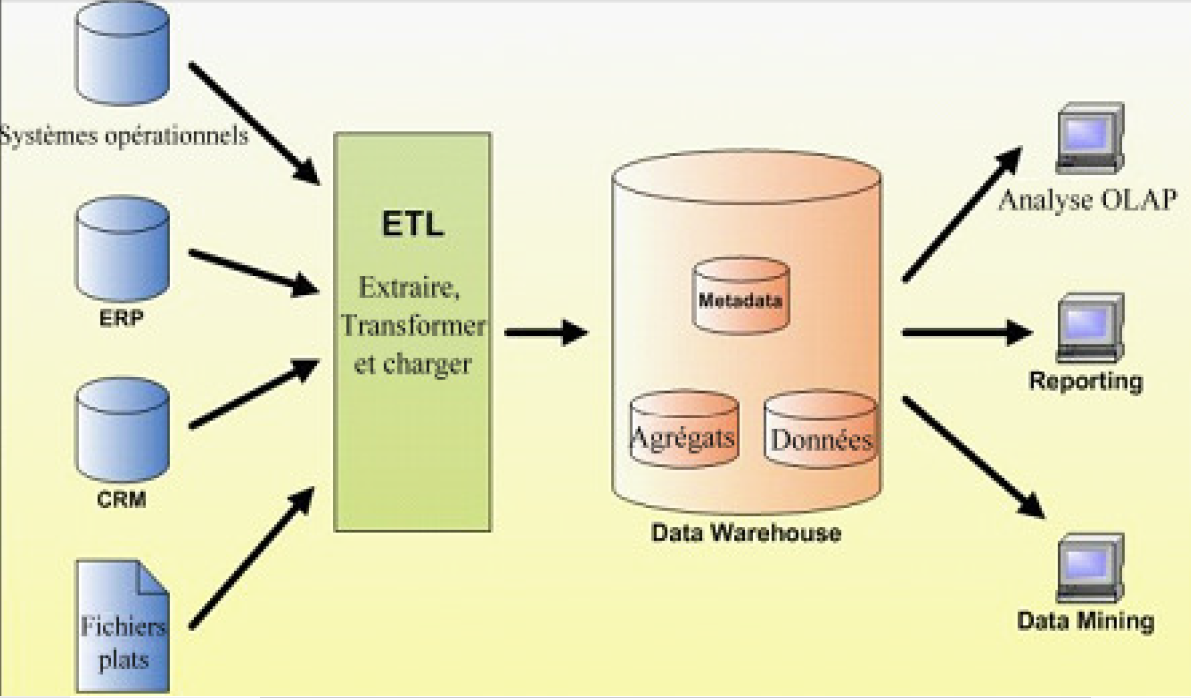
\includegraphics[scale=0.85]{images/DataWH.png}
		\caption{Architecture generale d'un data warehouse}
		\label{architecture-data-warehouse}
	\end{center}
\end{figure}

La figure ci-dessus Illustre la forme générale d’un data Warehouse que nous allons détailler dans les paragraphes suivants.

\textbf{Les Sources de données :} Dans la figure, les représentations de systèmes opérationnel, ERP, CRM et Fichiers plat font office de source de données et c’est d’elles qu’on puisse les données pour alimenter la machine décisionnelle.

\textbf{ETL (Extract, Transform, Load)}: C’est un ensemble de méthodes et d’outils qui servent a :\\
-	Extract : Extraire les données de sources hétérogènes\\
-	Transform : Transformation des données pour les mettre dans un format acceptable\\
-	Load : Charger les données dans le data warehouse\\

\textbf{Data Warehouse} : L’unité de stockage des données. Il est constitué de plusieurs éléments dont :\\ 
-	\textbf{Meta données} : ce sont les informations relatives à la structure des données, les méthodes d’agrégation et le lien entre les données opérationnelles et celles du Data Warehouse. Les métadonnées doivent renseigner sur :
 \begin{description}
 \item Le modèle de données,
 \item La structure des données telle qu’elle est vue par les développeurs,
 \item La structure des données telle qu’elle est vue par les utilisateurs,
 \item Les sources des données,
 \item Les transformations nécessaires,
 \item Suivi des alimentations,
 \end{description}
-	\textbf{Les Agrégats} (Données agrégées) : données agrégées à partir des données détaillées.\\

Les derniers éléments de la figure font partie de la phase d’exploitation du data warehouse et seront détaillés plus bas dans le document.


\section{Modélisation des données de l’entrepôt}

 \subsection{La modélisation dimensionnelle et ses concepts}
 	Les Data Warehouse sont destinés à la mise en place de systèmes décisionnels. Ces systèmes, devant répondre à des objectifs différents des systèmes transactionnels, ont fait ressortir très vite la nécessité de recourir à un modèle de données simplifié et aisément compréhensible. La modélisation dimensionnelle permet cela. Elle consiste à considérer un sujet d’analyse comme un cube à plusieurs dimensions, offrant des vues en tranches ou des analyses selon différents axes.
 	
 \begin{figure}[h]
	\begin{center}
		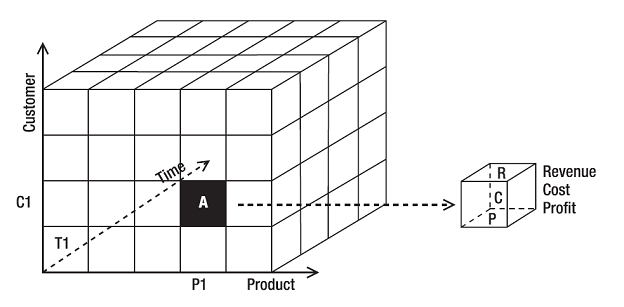
\includegraphics[scale=0.85]{images/cube.png}
		\caption{A cube with three dimensions.[ Rainardi 2008].}
		\label{Cube-dimensionnel}
	\end{center}
\end{figure}
 
 
 \subsubsection{Le concept des Faits}
 	 Une table de faits est la table centrale d’un modèle dimensionnel, où les mesures de performances sont stockées. Une ligne d'une table de faits correspond à une mesure. Ces mesures sont généralement des valeurs numériques, additives ; cependant des mesures textuelles peuvent exister mais sont rares. Le concepteur doit faire son possible pour faire des mesures textuelles des dimensions, car elles peuvent êtres corrélées efficacement avec les autres attributs textuels de dimensions.
 
 \subsubsection{Le concept des Dimensions}
 
  Les tables de dimension sont les tables qui raccompagnent une table de faits, elles contiennent les descriptions textuelles de l'activité. Une table de dimension est constituée de nombreuses colonnes qui décrivent une ligne. C'est grâce à cette table que l'entrepôt de données est compréhensible et utilisable; elles permettent des analyses en tranches et en dés. Une dimension est généralement constituée : d'une clé artificielle, une clé naturelle et des attributs.
  
 \subsection{Différents modèles de la modélisation dimensionnelle}
  
  \textbf{Modèle en étoile} : comme indiqué précédemment, ce modèle se présente comme une étoile dont le centre n’est autre que la table des faits et les branches sont les tables de dimension. La force de ce type de modélisation est sa lisibilité et sa performance. 
  
  \begin{figure}[h]
	\begin{center}
		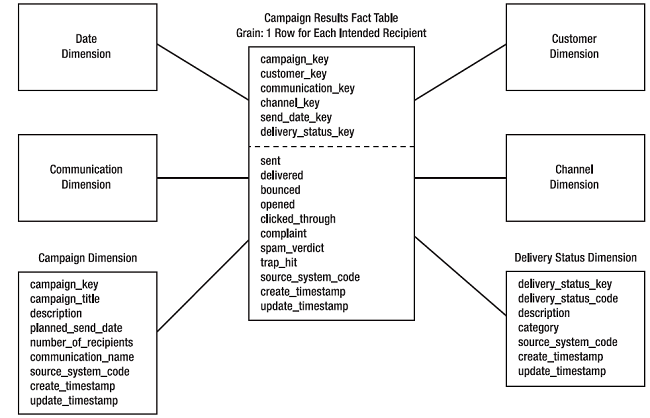
\includegraphics[scale=0.85]{images/etoile.png}
		\caption{Exemple d'un modèle en étoile « Dimensional star schema for campaign results data mart »[ Rainardi 2008]}
		\label{model-en-etoile}
	\end{center}
\end{figure}
\textbf{Modèle en flocon} : identique au modèle en étoile, sauf que ses branches sont éclatées en hiérarchies. Cette modélisation est généralement justifiée par l'économie d'espace de stockage, cependant elle peut s’avérer moins compréhensible pour l'utilisateur final, et très couteux en termes de performances.

\textbf{Modèle en constellation} : Ce n'est rien d'autre que plusieurs modèles en étoile liés entre eux par des dimensions communes.

  
  \subsection{La navigation dans les données}
  
  \paragraph{}
  Une fois que le serveur OLAP a construit le cube multidimensionnel « ou simulé ce cube selon l’architecture du serveur », plusieurs opérations sont possibles sur ce dernier offrant ainsi la possibilité de naviguer dans les données qui le constituent. Ces opérations de navigation « Data Surfing » doivent être, d’une part, assez complexes pour adresser l’ensemble des données et, d’autre part, assez simples afin de permettre à l’utilisateur de circuler de manière libre et intuitive dans le modèle dimensionnel.\\
  
Afin de répondre à ces attentes, un ensemble de mécanismes est exploité, permettant une navigation par rapport à la dimension et par rapport à la granularité d’une dimension.

  \subsubsection{Slice \& Dice}
  Le « Slicing » et le « Dicing » sont des techniques qui offrent la possibilité de faire des tranches « trancher » dans les données par rapport à des filtres de dimension bien précis, se classant de fait comme des opérations liées à la structure « se font sur les dimensions ». La différence entre eux se manifestent dans le fait que :\\
  
  \textit{Slicing is the process of retrieving a block of data from a cube by filtering on one dimension [Rainardi 2008].} 
   
   \begin{figure}[h]
	\begin{center}
		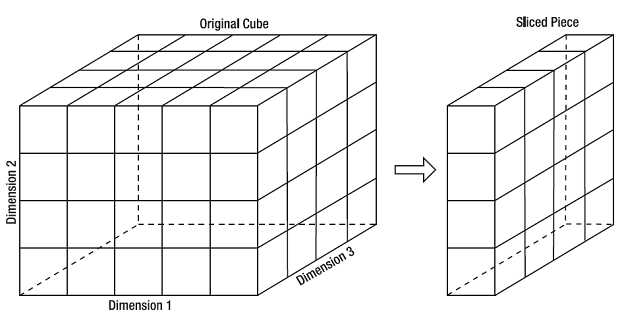
\includegraphics[scale=0.85]{images/slicing.png}
		\caption{Slicing}
		\label{slicing-image}
	\end{center}
   \end{figure}

\textit{Dicing is the process of retrieving a block of data from a cube by filtering on all dimensions [Rainardi 2008].}
  
    \begin{figure}[h]
	\begin{center}
		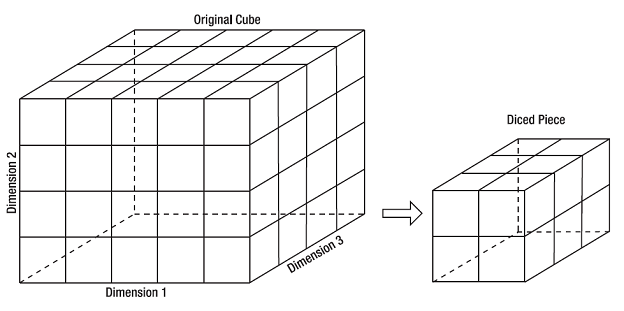
\includegraphics[scale=0.85]{images/dicing.png}
		\caption{Dicing}
		\label{slicing-image}
	\end{center}
   \end{figure}
   
   
   
\section{Démarche de Construction d’un Data Warehouse}   
   Plusieurs chercheurs ou équipes de recherche ont essayé de proposer des démarches pour la réalisation d’un projet Data Warehouse, ces démarches se croisent essentiellement dans les étapes suivantes :
\begin{list}{•}{ }
   \item Modélisation et conception du Data Warehouse,
   \item Alimentation du Data Warehouse,
   \item Mise en œuvre du Data Warehouse,
   \item Administration et maintenance du Data Warehouse,\\
\end{list}

\subsection{Modélisation et conception du Data Warehouse}

Les deux approches les plus connues dans la conception des Data Warehouse sont :
\begin{list}{•}{ }
   \item L’approche basée sur les besoins d’analyse,
    \item L’approche basée sur les sources de données,\\
\end{list}
Aucune des deux approches citées n’est ni parfaite, ni applicable à tous les cas. Toutes deux doivent être étudiées pour choisir celle qui s’adapte le mieux à notre cas. Quel que soit l’approche adoptée pour la conception d’un Data Warehouse, la définition de celui-là reste la même. En étant un support d’aide à la décision, le Data Warehouse se base sur une architecture dimensionnelle.


 \subsubsection{Approche « Besoins d’analyse »}
 
  Le contenu du Data Warehouse sera déterminé selon les besoins de l’utilisateur final. Cette approche est aussi appelée « approche descendante » (Top-Down Approach) et est illustrée par R. Kimball grâce à son cycle de vie dimensionnel comme suit :
  
  \begin{figure}[h]
	\begin{center}
		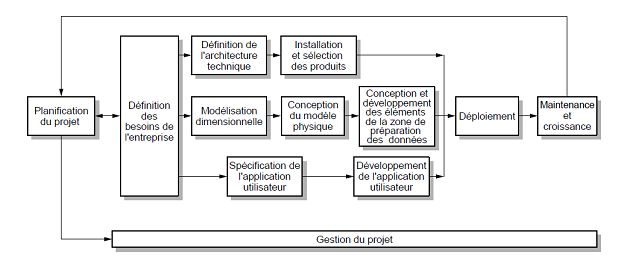
\includegraphics[scale=0.85]{images/besion_analyse.png}
		\caption{illustration de l’approche « Besoins d’analyse » grâce au cycle de vie dimensionnel de Kimball [Kimball, 2004].}
		\label{synthese-cout-salarie}
	\end{center}
\end{figure}

\begin{flushleft}
	\begin{longtable}{|p{0.5\textwidth}|p{0.5\textwidth}|}
		\caption{Avantages et inconvénients de l'approche « Besoins d’analyse »} 
		\label{Transactionel vs descisionel}
		\\
		
		
		\hline 
		\textbf{Avantages} &
		\textbf{Inconvénients}
		\\
		
		\hline
		\endhead
		\hline
		\endfoot
		\hline
		 
		\begin{description}
		 \item Aucun risque de concevoir une solution obsolète avant d’être opérationnelle
		 \end{description}
		  &
		 
	   \begin{description}
		\item  Pas de prise en compte de l’évolution des besoins de l’utilisateur.
		\item Nécessite une modification de la structure du Data Warehouse en cas de nouveau besoin
		\item Négligence du système opérationnel
		\item Difficulté de déterminer les besoins des utilisateurs
		\end{description}
		\\ 	
		\hline 
	\end{longtable} 
\end{flushleft}


\subsubsection{Approche « Source de données »}
Le contenu du Data Warehouse est déterminé selon les sources de données. Cette approche est appelée: Approche ascendante (Bottom-up Approach).

  \begin{flushleft}
	\begin{longtable}{|p{0.5\textwidth}|p{0.5\textwidth}|}
		\caption{Avantages et inconvénients de l'approche « Besoins d’analyse »} 
		\label{Transactionel vs descisionel}
		\\
		
		
		\hline 
		\textbf{Avantages} &
		\textbf{Inconvénients}
		\\
		
		\hline
		\endhead
		\hline
		\endfoot
		\hline
		 
		\begin{description}
		 \item Meilleure prise en charge de l’évolution des besoins
		 \end{description}
		  &
		 
	   \begin{description}
		\item  Risque de concevoir une solution obsolète avant qu’elle soit opérationnelle
		\item Evolution du schéma des données source
		\item Complexité de source de données
		\end{description}
		\\ 	
		\hline 
	\end{longtable} 
\end{flushleft}


\paragraph{•}
Inmon considère que l’utilisateur ne peut jamais déterminer ses besoins dès le départ, « Donnez-moi ce que je vous demande, et je vous direz ce dont j’ai vraiment besoin », il considère que les besoins sont en constante évolution.

\subsubsection{Approche mixte}
\paragraph{}
Une combinaison des deux approches appelée hybride ou mixte peut s’avérer efficace. Elle prend en considération les sources de données et les besoins des utilisateurs.\\

Cette approche consiste à construire des schémas dimensionnels à partir des structures des données du système opérationnel, et les valider par rapport aux besoins analytiques. Cette approche cumule les avantages et quelques inconvénients des deux approches déjà citées, telles que la complexité des sources de données et la difficulté quant à la détermination des besoins analytiques.


\subsection{Les phases de l'alimentation « E.T.L »}

Les phases du processus E.T.L. représentent la mécanique d’alimentation du Data
Warehouse. Ainsi elles se déroulent comme suit :\\
\textbf{a) L’extraction des données}\\

\textit{« L’extraction est la première étape du processus d’apport de données à l’entrepôt de données. Extraire, cela veut dire lire et interpréter les données sources et les copier dans la zone de préparation en vue de manipulations ultérieures. »} [Kimball, 2005]. Elle consiste en :\\

 •	Cibler les données,\\
 •	Appliquer les filtres nécessaires,\\
 •	Définir la fréquence de chargement\\

Lors du chargement des données, il faut extraire les nouvelles données ainsi que les changements intervenus sur ces données. Pour cela, il existe trois stratégies de capture de changement :\\
• Colonnes d’audit : la colonne d’audit, est une colonne qui enregistre la date d’insertion ou du dernier changement d’un enregistrement. Cette colonne est mise à jour soit par des triggers ou par les applications opérationnelles, d’où la nécessité de vérifier leur fiabilité.\\
\quad •	Capture des logs : certains outils ETL utilisent les fichiers logs des systèmes sources afin de détecter les changements (généralement logs du SGBD). En plus de l’absence de cette fonctionnalité sur certains outils ETL du marché, l’effacement des fichiers logs engendre la perte de toute information relative aux transactions.\\
\qquad • Comparaison avec le dernier chargement : le processus d’extraction sauvegarde des copies des chargements antérieurs, de manière à procéder à une comparaison lors de chaque nouvelle extraction. Il est impossible de rater un nouvel enregistrement avec cette méthode.


\begin{figure}[h]
	\begin{center}
		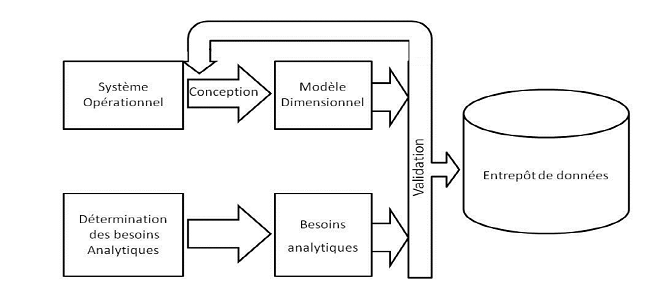
\includegraphics[scale=0.85]{images/mixte.png}
		\caption{Illustration de l’approche mixte.}
		\label{synthese-cout-salarie}
	\end{center}
\end{figure}

\textbf{b) La transformation des données}

La transformation est la seconde phase du processus. Cette étape, qui du reste est très importante, assure en réalité plusieurs tâches qui garantissent la fiabilité des données et leurs qualités. Ces tâches sont :\\
•	Consolidation des données.\\
•	Correction des données et élimination de toute ambiguïté.\\
•	Élimination des données redondantes.\\
•	Compléter et renseigner les valeurs manquantes. Cette opération se solde par la production d’informations dignes d’intérêt pour l’entreprise et de et sont donc prêtes à être entreposées.\\

\textbf{c) Le chargement des données}

C’est la dernière phase de l’alimentation d’un entrepôt de données, le chargement est une étape indispensable. Elle reste toutefois très délicate et exige une certaine connaissance des structures du système de gestion de la base de données (tables et index) afin d’optimiser au mieux le processus.

\subsubsection{Politiques de l’alimentation}
\paragraph{}
Le processus de l’alimentation peut se faire de différentes manières. Le choix de la politique de chargement dépend des sources : disponibilité et accessibilité. Ces politiques
sont8 :\\
\textbf{• Push} : dans cette méthode, la logique de chargement est dans le système de production. Il " pousse " les données vers la zone de préparation quand il en a l'occasion. L'inconvénient est que si le système est occupé, il ne poussera jamais les données.\\
\textbf{• Pull} : contrairement de la méthode précédente, le Pull " tire " les données de la source vers la zone de préparation. L'inconvénient de cette méthode est qu'elle peut surcharger le système s'il est en cours d'utilisation.\\
\textbf{• Push-pull} : c'est la combinaison des deux méthodes. La source prépare les données à envoyer et indique à la zone de préparation qu'elle est prête. La zone de préparation va alors récupérer les données.
Les Processus ETL doit respecter les critères suivants\\
\textbf{Sûr }: assure l’acheminement des données et leur livraison.
Rapide : la quantité de données manipulées peut causer des lenteurs. Le processus d’alimentation doit palier à ce problème et assurer le chargement du Data Warehouse dans des délais acceptables.\\
\textbf{Correctif }: le processus d’alimentation doit apporter les correctifs nécessaires pour améliorer la qualité des données.\\
\textbf{Transparent} : le processus de l’ETL doit être transparent afin d’améliorer la qualité des données.


\subsection{Mise en œuvre du Data Warehouse}
  C’est la dernière étape d’un projet Data Warehouse, soit son exploitation. L’exploitation du Data Warehouse se fait par le biais d’un ensemble d’outils analytiques développés autour du Data Warehouse. Donc cette étape nécessite l’achèvement du développement, ou de la mise en place, de ces outils qui peuvent accomplir les fonctions suivantes:\\
  
 \textbf{a. Requêtage ad-hoc}\\ 
  Le requêtage ad-hoc reste très fréquent dans ce type de projet. En effet, les utilisateurs de l’entrepôt de données, et spécialement les analystes, seront amenés à interagir avec le DW via des requêtes ad-hoc dans le but de faire les analyses requises par leurs métiers et, d’élaborer aussi, des rapports et des tableaux de bords spécifiques. L’accès à ce genre de service peut se faire via différentes méthodes et outils. Cependant, les spécialistes en la matière préconisent de laisser la possibilité à l’utilisateur de choisir les outils qui lui paraissent les plus adéquats.
  
 \textbf{ b. Reporting :}\\
Destiné essentiellement à la production de rapports et de tableaux de bord, \textit{« il est la présentation périodique de rapports sur les activités et résultats d'une organisation, d'une unité de travail ou du responsable d'une fonction, destinée à en informer ceux chargés de les superviser en interne ou en externe, ou tout simplement concernés par ces activités ou résultants »[ http://fr.wikipedia.org/wiki/Reporting].}\\

Ces outils de Reporting ne sont pas, à proprement parler, des instruments d'aide à la décision, mais, lorsqu’ils sont utilisés de manière appropriée, ils peuvent fournir une précieuse vue d’ensemble.\\

Les rapports sont alors crées par le biais d’outils de Reporting qui permettent de leur donner un format prédéterminé. Les requêtes sont constituées lors de l’élaboration des rapports qui seront ensuite diffusés périodiquement en automatique ou ponctuellement à la demande.\\


\textbf{d. Tableaux de bord :}\\
Les tableaux de bord sont un outil de pilotage qui donne une vision sur l’évolution d’un processus, afin de permettre aux responsables de mettre en place des actions correctives.\\
\textit{« Le tableau de bord est un ensemble d’indicateurs peu nombreux conçus pour permettre aux gestionnaires de prendre connaissance de l’état et de l’évolution des systèmes qu’ils pilotent et d’identifier les tendances qui les influenceront sur un horizon cohérent avec la nature de leurs fonctions » [Bouquin, 2003]}.\\
Cette forme de restitution a la particularité de se limiter à l’essentiel, c'est-à-dire la mise en évidence de l’état d’un indicateur par rapport à un objectif, tout en adoptant une représentation graphique de l’information.\\

\textbf{e. Data Mining :}\\
Au sens littéral du terme, le Data Mining signifie le forage de données. Le but de ce forage est d’extraire de la matière brute qui, dans notre cas, représente de nouvelles connaissances. L’idée de départ veut qu’il existe dans toute entreprise des connaissances utiles, cachées sous des gisements de données. Le Data Mining permet donc, grâce à un certain nombre de techniques, de découvrir ces connaissances en faisant apparaître des corrélations entre ces données.\\
Le Data Warehouse constituera alors la première source de données sur laquelle s’exécutera le processus de découverte de connaissances. Dans la majeure partie du temps, l’entrepôt de données représente un pré requis indispensable à toute fouille de données.\\
Le recours à ce genre de méthode est de plus en plus utilisé dans les entreprises modernes. Les applications et outils implémentant ces solutions sont rarement développés en interne. En effet, les entreprises préfèrent se reposer sur des valeurs sûres du marché afin d’exploiter au plus vite les données en leur possession.

 \subsection{Maintenance et expansion}
 La mise en service du Data Warehouse ne signifie pas la fin du projet, car un projet
Data Warehouse nécessite un suivi constant compte tenu des besoins d’optimisation de performance et ou d’expansion. Il est donc nécessaire d’investir dans les domaines suivants:\\
\textbf{Support} : assurer un support aux utilisateurs pour leur faire apprécier l’utilisation de l’entrepôt de données. En outre, la relation directe avec les utilisateurs permet de détecter les  correctifs nécessaires à apporter.\\
\textbf{Formation} : il est indispensable d’offrir un programme de formation permanant aux utilisateurs de l’entrepôt de données.\\
Support technique : un entrepôt de données est considéré comme un environnement de production. Naturellement le support technique doit surveiller avec la plus grande vigilance les performances et les tendances en ce qui concerne la charge du système.\\
\textbf{Management de l’évolution}: il faut toujours s’assurer que l’implémentation répond aux besoins de l’entreprise. Les revues systématiques à certain point de contrôle sont un outil clé pour détecter et définir les possibilités d’amélioration. En plus du suivi et de la maintenance du Data Warehouse, des demandes d’expansion sont envisageables pour de nouveaux besoins, de nouvelles données ou pour des améliorations.
Ces travaux d’expansion sont à prévoir de façon à faciliter l’évolution du schéma du
Data Warehouse.


%\begin{figure}[h]
%	\begin{center}
%		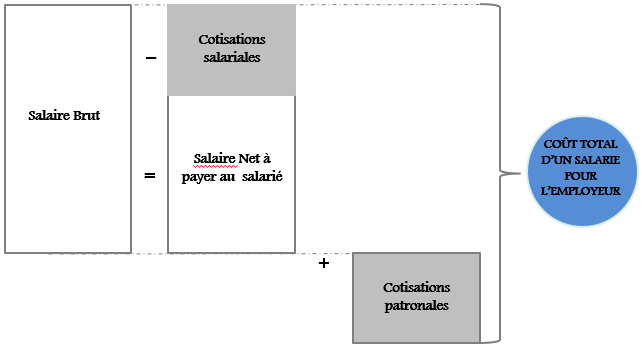
\includegraphics[scale=0.85]{images/remuneration.png}
%		\caption{Schéma de synthèse sur le coût d'un salarié}
%		\label{synthese-cout-salarie}
%	\end{center}
%\end{figure}



\chapter{Titre du chapitre}     % numéroté

Texte du chapitre.


\part{CONTRIBUTION}

\chapter{Titre du chapitre}     % numéroté

Texte du chapitre.

\chapter{titre}














\chapter{ANALYSE ET CONCEPTION}

\section{ANALYSE}
Une fois les besoins des utilisateurs connu, nous pouvons commencer à concevoir les volets de notre data warehouse. Pour cela, nous avons eu recours à la modélisation dimensionnelle qui est souvent associé aux entrepôts de données compte tenu de ses avantages.
Cependant, avant de se lancer dans la modélisation il est intéressant de classer les sujets récence selon la pertinence pour l’entreprise et la facilité de réalisation. Ce classement nous aidera à choisir l’activité à modéliser en premier lieu de manière à garantir des résultats satisfaisants pour l’entreprise.\\

\subsection{PROCESSUS DE MODÉLISATION}
 
 La conception d’un modèle dimensionnel passe par cinq étapes essentielles :
 \begin{list}{•}{ }
    \item Choix de l’activité a modéliser : ce choix se fait après classement des activités dans une matrice dite d’analyse des priorités [Kimball, 2004]. Cette matrice permet de connaître quelle activité choisir en premier. Le classement des sujets recensés, qui s’est fait en collaboration avec les décideurs de l’entreprise est illustre dans la figure suivante.
    \begin{figure}[!htbp]
	\begin{center}
		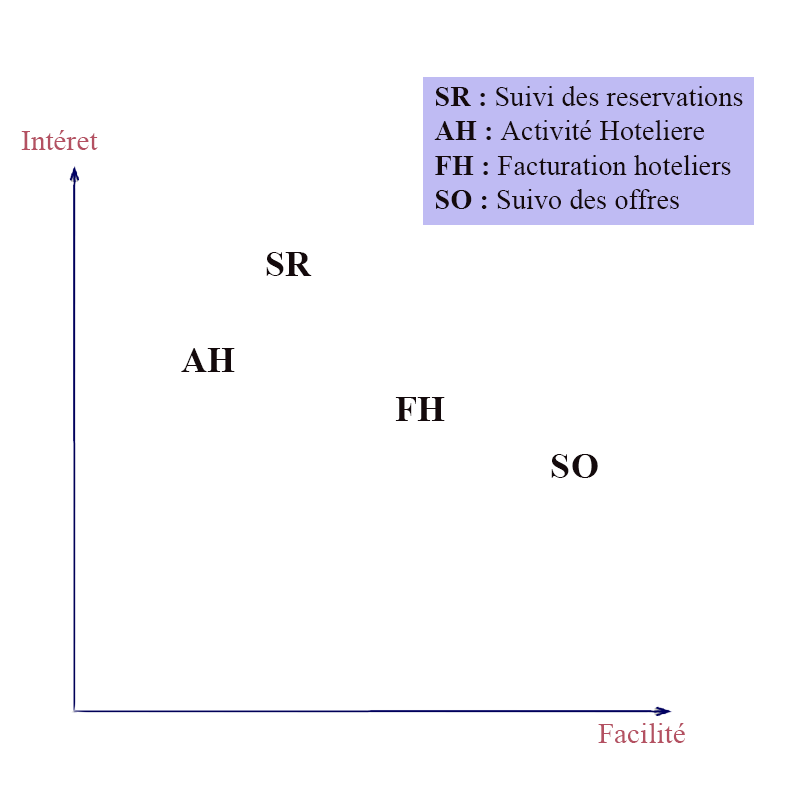
\includegraphics[scale=0.40]{images/priority.png}
		\caption{Analyse des priorités de Hosteline.}
		\label{use_bi_tools}
	\end{center}
	\end{figure}
    \item Définition de l’activité et de son grain
	\item Définition des dimensions qui décrivent une ligne de la table de fait
	\item Définir les mesurables du fait
    \item Définir les agrégats 
    
 \end{list}
 

\subsubsection{Volet « Réservation »}

\textbf{a)	Présentation de l’activité “Réservation”}\\
Selon Larousse, Une réservation est  \textit{l’action de retenir une place (dans un train, un avion, au théâtre, etc.), une table (au restaurant), une chambre (dans un hôtel)}.\\
La réservation sur Hosteline est au cœur de son activité réalisant la majorité de son chiffre d’affaire. Les chiffres lies à la réservation se présentent comme des indicateurs de grande signification par rapport a l’activité de l’entreprise. Ainsi la disponibilité de ces informations s’avère indispensable pour les décideurs de l’entreprise.\\

\textbf{b)	Grain de l’activité}\\
Le choix du grain le plus fin donne un maximum de flexibilité. Dans le cas des réservations le grain le plus fin, ou le niveau de détail le plus bas, correspond à une opération de réservation.

\textbf{c)	Dimensions participantes}\\
Les dimensions ont pour objectif de décrire un fait, Donc pour ce cas on essaye de recenser les informations qui décrivent au mieux une réservation.\\

\textbf{1 Dimension Temps}
La dimension temps est \textit{« la seul dimension qui figure systématiquement dans tout entrepôt de données, car en pratique tout entrepôt de données est une série temporelle. Le temps est le plus souvent la première dimension sou jacent de la base de données »} [Kimball, 2001]\\

La dimension temps se présente comme suit :

\begin{figure}[!htbp]
	\begin{center}
		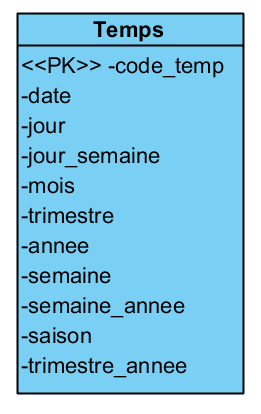
\includegraphics[scale=0.65]{images/dim_temps.png}
		\caption{Dimension temps du volet "Réservation".}
		\label{use_bi_tools}
	\end{center}
	\end{figure}

Le niveau de détail le plus bas de cette dimension est la journée. En effet, les utilisateurs ont fait ressortir le besoin de suivre les chiffres au jour le jour et d’en garder l'historique de ces derniers\\
Dans cette dimension, il est utilisé une clé artificielle comme clé primaire. Cette clé artificielle sert à faciliter la manipulation de la dimension.\\

\textbf{2 Dimension Client}\\
Le client s’impose comme un élément important dans l’analyse et intéresse les analystes et les décideurs de l’entreprise. Outre ce qu’il représente dans une opération de vente, l’analyse du comportement du client peut aider l’entreprise à mieux le satisfaire. La dimension client décrit un client, la personne qui réserve un hébergement.

\begin{figure}[!htbp]
	\begin{center}
		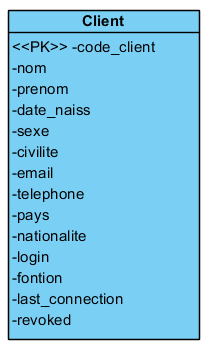
\includegraphics[scale=0.65]{images/dim_client.png}
		\caption{Dimension client du volet "Réservation".}
		\label{use_bi_tools}
	\end{center}
	\end{figure}

\textbf{3 Dimension Hôtel}
La réservation présentée plus haut est une convention entre un client et un hôtel. D’où le besoin d’une dimension hôtel. Cette dimension propose des axes d'analyses de grande importance déclinée dans la figure qui suit.
\cleardoublepage
\begin{figure}[!htbp]
	\begin{center}
		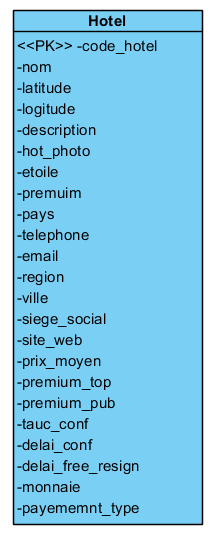
\includegraphics[scale=0.65]{images/dim_hotel.png}
		\caption{Dimension hotel du volet "Réservation".}
		\label{use_bi_tools}
	\end{center}
\end{figure}


\textbf{d) Les mesurables}\\
Les mesurables qui correspondent à l’activité des réservations et qui permettent de mesurer les performances de cette activité, sont la \textit{« Le CA des promotions \(CA\_res\_promo\) », « montant total des réservations \(CA\_reservation\) », «nombre de personne \(nbre\_personnes\)»}  et le \textit{« nombre de nuits \(nbre\_nuits\) »}.

\begin{figure}[!htbp]
	\begin{center}
		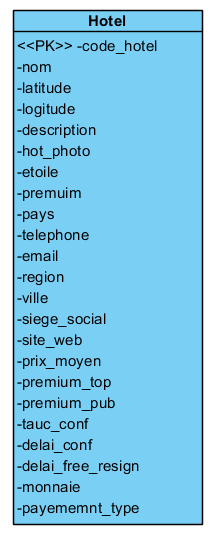
\includegraphics[scale=0.65]{images/dim_hotel.png}
		\caption{Table des faits du volet "Réservation".}
		\label{use_bi_tools}
	\end{center}
	\end{figure}

e) Le modèle en étoile de l’activité « Réservations »

\begin{figure}[!htbp]
	\begin{center}
		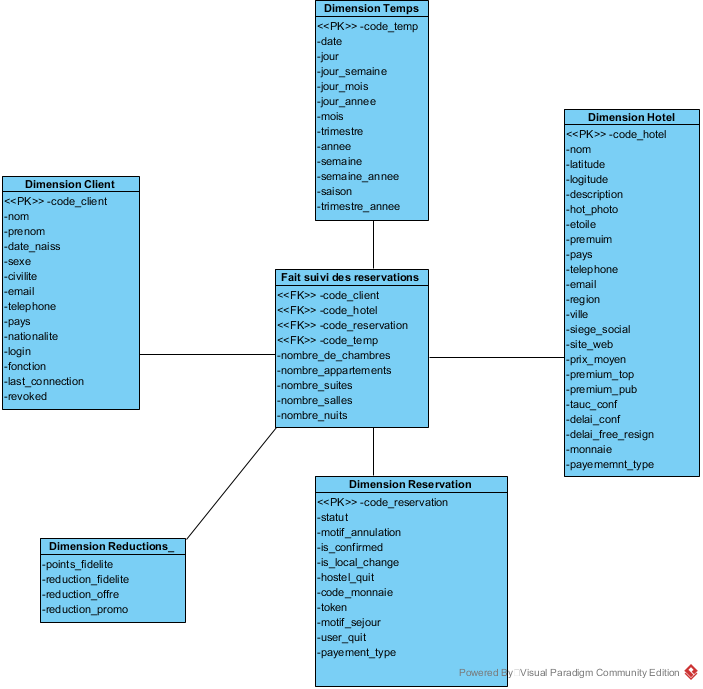
\includegraphics[scale=0.65]{images/star_reservations.png}
		\caption{Modèle en étoile du volet "Réservation".}
		\label{use_bi_tools}
	\end{center}
	\end{figure}

\textbf{f) Les agrégats}\\
Les tables d’agrégats améliorent les performances du Data Warehouse, en réduisant le nombre de lignes que le SGBD manipule afin de répondre à une requête. Cela se fait grâce à l’agrégation des données contenues dans les tables de faits détaillées et qui sont stockées dans de nouvelles tables de faits.
La construction des agrégats se base sur le modèle en étoile détaillée, et elle peut nécessiter:
\begin{list}{•}{ }
   \item La création de nouvelles dimensions dérivées : la construction d’un modèle agrégé nécessitera la suppression de quelques attributs d’une dimension qui désigne le grain le plus fin.
   \item La suppression de quelques dimensions : le modèle agrégé peut engendrer l’élimination de certaines dimensions qui n’apparaissent pas au niveau de détail voulu. On peut aussi :
   \item Créer de nouveaux faits: lors de la création de la table de faits agrégée on peut rajouter quelques faits qui n’existaient pas dans la modèle de base. En effet, l’usage et la signification des tables agrégées peuvent différer du modèle de base.
   \item  Créer des tables pré-jointes : une table d’agrégat peut être construite à partir d’une jointure entre la table de faits et une ou plusieurs dimensions. Le résultat est stocké dans une seule table dite pré-jointure. Une table d’agrégat peut être invisible ou visible à l’utilisateur final :
 \begin{list}{-}{ }
       \item Elle est invisible lorsqu’elle reflète exactement le modèle de base
       \item Elle est visible lorsqu’elle contient des faits supplémentaires.
 \end{list}
Les résultats issus d’une table agrégée ou du modèle de base doivent être identique.
Pour cette phase, on s’inspire de la démarche décrite par C. Adamson dans son livre
« Mastering the Data Warehouse Aggregates, Solution for Star Schema Performance ». La démarche consiste à :
\begin{enumerate}
 \item Enumérer les agrégats potentiels à partir d’une étoile détaillée : pour détecter les agrégats potentiels et choisir ceux à implémenter dans le Data Warehouse. Il est nécessaire de bien décrire chaque agrégat.
  \item Détecter les agrégats utiles : choisir des agrégats utiles à partir des agrégats potentiels.
  \item Construire le modèle agrégé : enfin on construit le modèle agrégé tout en prenant en considération les dimensions dérivées commune entre les différents modèles.
\end{enumerate}
\end{list}

\textbf{1- Les agrégats potentiels}

\begin{figure}[!htbp]
	\begin{center}
		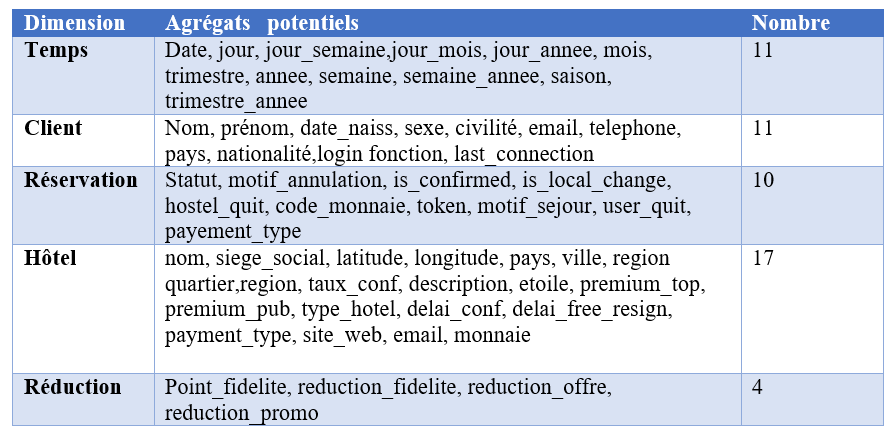
\includegraphics[scale=0.65]{images/tab_agregat_pot_reservation.png}
		\caption{Les agrégats potentiels du volet "Réservation".}
		\label{use_bi_tools}
	\end{center}
	\end{figure}
\cleardoublepage
\textbf{2	Les agrégats utiles}
\begin{figure}[!htbp]
	\begin{center}
		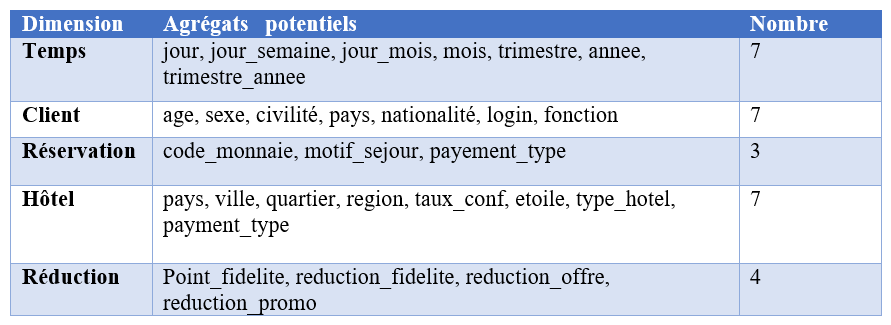
\includegraphics[scale=0.65]{images/tab_agregat_uti_reservation.png}
		\caption{Les agrégats utiles du volet "Réservation".}
		\label{use_bi_tools}
	\end{center}
	\end{figure}

A partir du tableau précédent nous choisissons les agrégats qui nous semblent les plus pertinents et susceptibles de faire l’objet d’accès fréquents. Nous arrêtons la liste des modèles agrégats suivants :
\begin{list}{•}{ }
\item Réservations journalières selon le lieu de provenance du client
\item Réservations journalières par nombre d’étoiles de l’hôtel
\item Taux de réservations par rapport aux réductions offertes.
\end{list}

 \subsubsection{Volet OFFRES}
\textbf{a)	Présentation des Offres}\\

Les offres constituent un des arguments marketing que possède la plateforme. Une offre est un pack constitué d’un ensemble d’hébergements et d’autres 

\textbf{b)	Grain de l’activité}\\
Le grain le plus fin de l’activité hôtelière correspond à : 
\begin{center}
\textit{Suivi des demandes faites à un hôtel à un endroit selon les réductions qu’il offre a une date donnée.}
\end{center}
\cleardoublepage
\textbf{f)	Les dimensions participantes du model}\\

Après la détection des dimensions de la nouvelle étoile, on procède à une mise en conformité des dimensions communes. Pour ce faire, on construit un tableau qui croise les étoiles conçues avec leurs dimensions. Le but étant de détecter les dimensions communes pour leurs mises en conformité. Le tableau suivant illustre cela.

\begin{figure}[!htbp]
	\begin{center}
		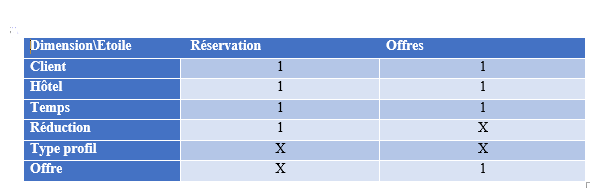
\includegraphics[scale=0.95]{images/tab_conform.png}
		\caption{Comparaison des volet Réservations et Offres.}
		\label{use_bi_tools}
	\end{center}
	\end{figure}

\textbf{Dimension Offre}\\]
 Cette dimension est primordiale pour une appréciation juste des indicateurs de ce modèle. Les axes d’étude qu’offre cette dimension sont mis en relief dans la figure qui suit. 

\begin{figure}[!htbp]
	\begin{center}
		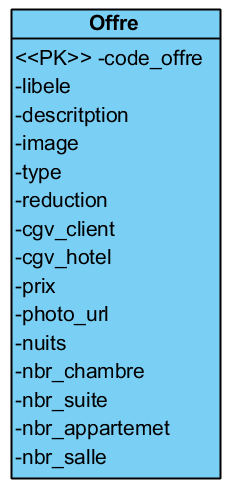
\includegraphics[scale=0.65]{images/dim_offre.png}
		\caption{Dimension offre du volet Offres.}
		\label{use_bi_tools}
	\end{center}
	\end{figure}
	
\cleardoublepage
\textbf{e) Le modèle en Etoile de l’activité « Suivi des Offres »}\\

\begin{figure}[!htbp]
	\begin{center}
		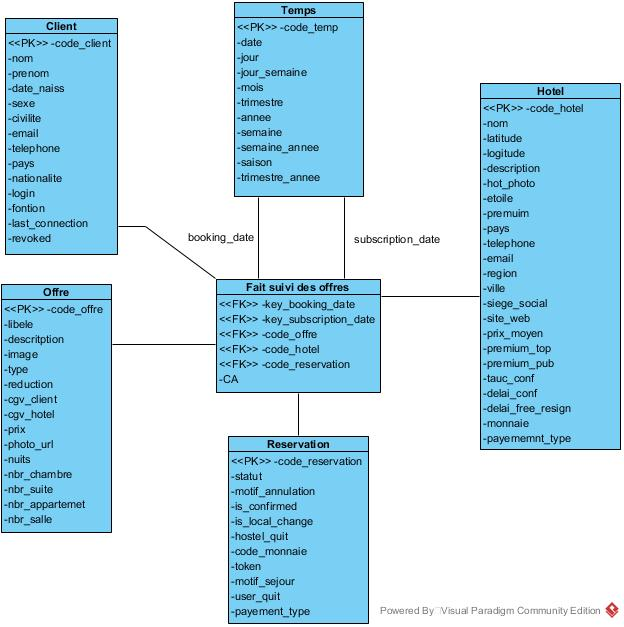
\includegraphics[scale=0.55]{images/star_offres.png}
		\caption{Modèle en étoile du volet "Offres".}
		\label{use_bi_tools}
	\end{center}
	\end{figure}


\textbf{1- Les agrégats potentiels}

\begin{figure}[!htbp]
	\begin{center}
		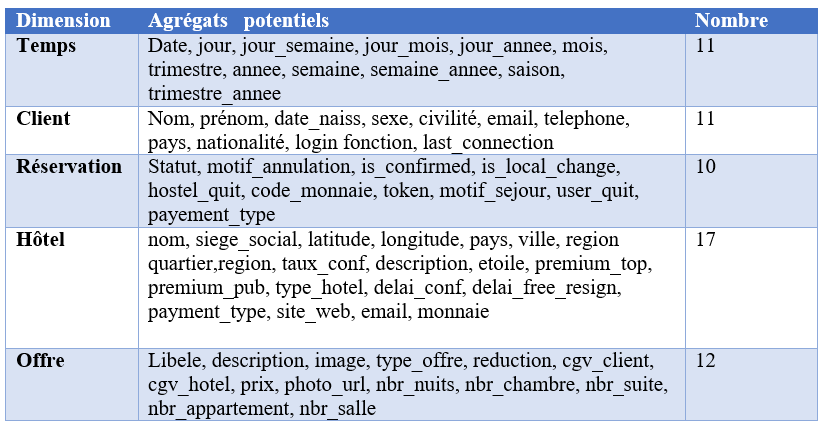
\includegraphics[scale=0.65]{images/tab_agregat_pot_offre.png}
		\caption{Les agrégats potentiels du volet "Offre".}
		\label{use_bi_tools}
	\end{center}
	\end{figure}
\cleardoublepage
\textbf{2	Les agrégats utiles}
\begin{figure}[!htbp]
	\begin{center}
		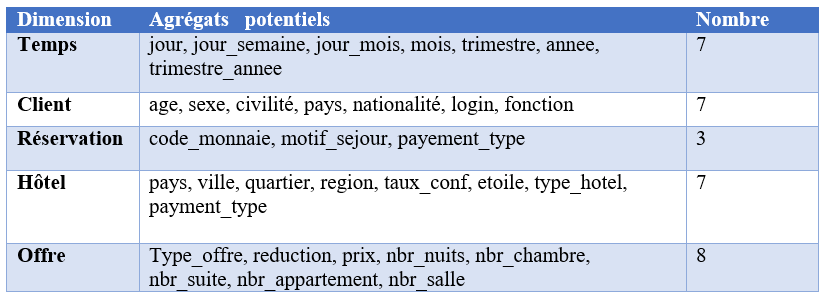
\includegraphics[scale=0.65]{images/tab_agregat_uti_offre.png}
		\caption{Les agrégats utiles du volet "Offre".}
		\label{use_bi_tools}
	\end{center}
	\end{figure}
	 
\section{CONCEPTION}


 


Afin de faciliter l'analyse et la navigation dans les données, il est important que les cubes dimensionnels soient bien conçues et définis de manière claire pour une utilisation intuitive.\\

    La conception des cubes dimensionnels passe par la définition des mesurables et des dimensions. Le but de la mise en place de ces cubes est d’offrir une représentation abstraite d'informations multidimensionnelles à des fins d’analyse. 


\subsection{Liste des cubes}
Dans ce qui suit nous allons dresser la liste des cubes à mettre en place. Pour chaque
cube on donnera les dimensions participantes ainsi que les mesurables présents dans ces
cubes.



	\begin{longtable}{|p{0.15\textwidth}|p{0.35\textwidth}|p{0.4\textwidth}|}
		\caption{Liste des cubes dimensionnels.} 
		\label{Liste des cubes dimensionnels}
		\\
		
		
		\hline 
		\textbf{Nom du cube} & 
		\textbf{Mesurables (Indicateurs)} &
		\textbf{Dimensions}
		\\
		
		
		\endfirsthead
		\caption[]{Liste des cubes dimensionnels (suite).} 
		\\
		\hline 
		\textbf{Nom du cube} & 
		\textbf{Mesurables (Indicateurs)} &
		\textbf{Dimensions}
		\\
		\hline
		\endhead
		\hline
		\endfoot
		\hline
		
		
		\hline
		Reservation &  
		
		\begin{description}
		 \item ca\_plateforme
		 \item ca\_hotel
		 \end{description} &
		 
		 \begin{description}
		 \item client
		 \item temps
		 \item type\_profile
		 \item reductions
		 \end{description}
		\\ 
		
		\hline
		Suivi des Offres &  
		\begin{description}
		 \item ca\_plateforme
		 \item nombre\_hotels
		 \item nombre\_reservations
		 \end{description} &
		\begin{description}
		 \item offre
		 \item temps
		 \item reservation
		 \item hotel
		 \item client
		 \end{description}
		\\
		
		\hline
		Suivi des hoteliers &  
		\begin{description}
		 \item ca\_reservation
		 \item ca\_reservation\_promo
		 \item nombre\_nuits
		 \item nombre\_nuitée
		 \item nombre\_chambre\_hotel
		 \end{description} &
		\begin{description}
		 \item temps
		 \item reservation
		 \item hotel
		 \item client
		 \item reductions
		 \end{description}
		\\  
		
		\hline
		facturation hotel &  
		\begin{description}
		 \item nombre\_hotels
		 \end{description} &
		\begin{description}
		 \item temps
		 \item reduction
		 \item hotel
		 \item client
		 \item type\_profile
		 \end{description}
		\\
		
		\hline
		Suivi des Offres &  
		\begin{description}
		 \item ca\_plateforme
		 \item nombre\_hotels
		 \item nombre\_reservations
		 \end{description} &
		\begin{description}
		 \item offre
		 \item temps
		 \item reservation
		 \item hotel
		 \item client
		 \end{description}
		\\
		
		\hline 
	\end{longtable} 

\cleardoublepage
\subsection{PRÉSENTATION DES DIMENSIONS}
\begin{figure}[!htbp]
	\begin{center}
		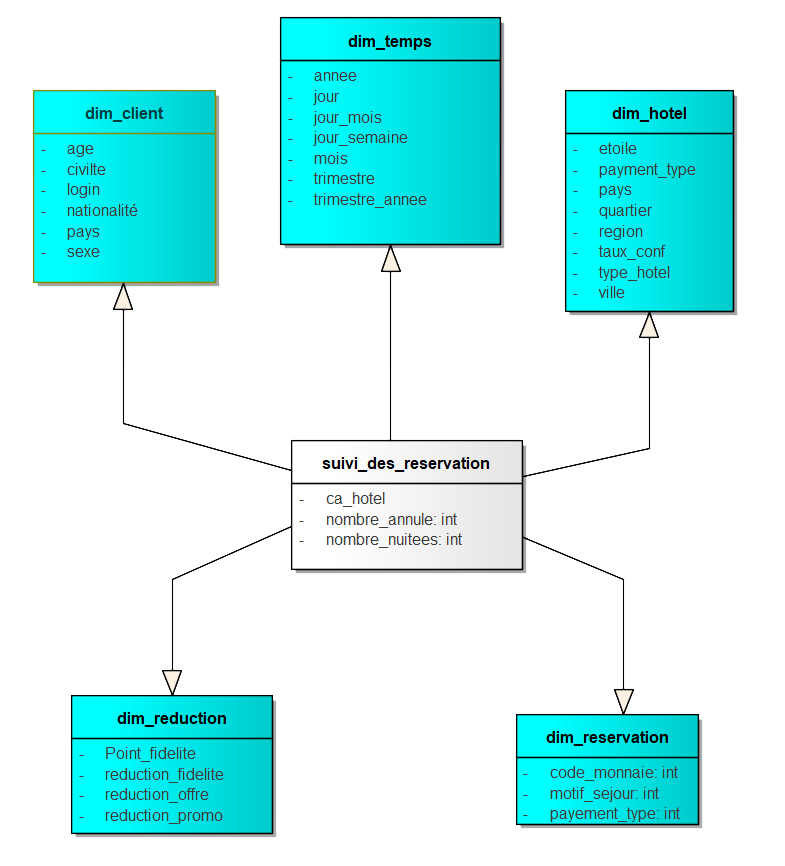
\includegraphics[scale=0.85]{images/cube_reservation.png}
		\caption{Cube dimensionnel « Suivi des reservations ».}
		\label{use_bi_tools}
	\end{center}
\end{figure}

\begin{figure}[!htbp]
	\begin{center}
		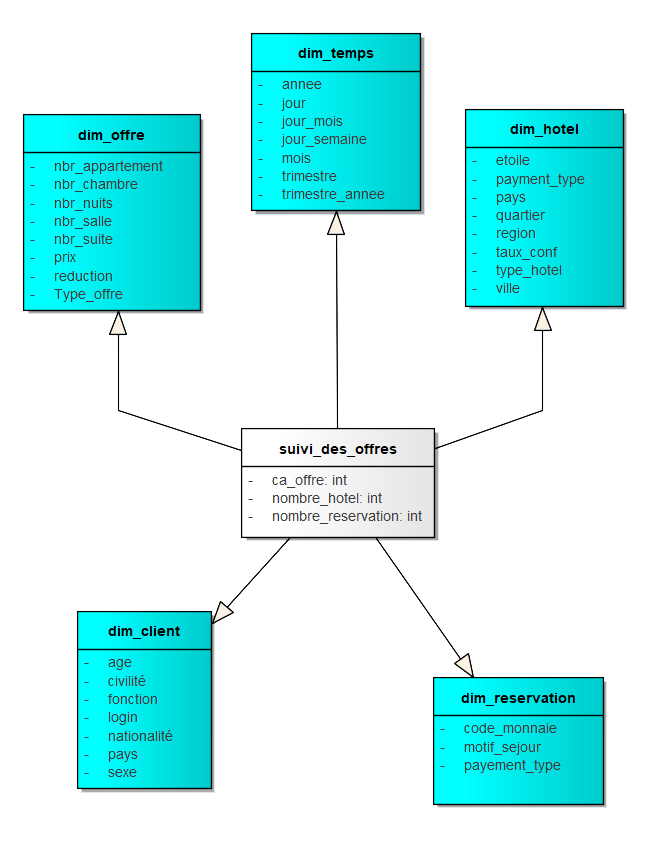
\includegraphics[scale=0.85]{images/cube_offre.png}
		\caption{Cube dimensionnel « Suivi de offres ».}
		\label{use_bi_tools}
	\end{center}
\end{figure}

\begin{figure}[!htbp]
	\begin{center}
		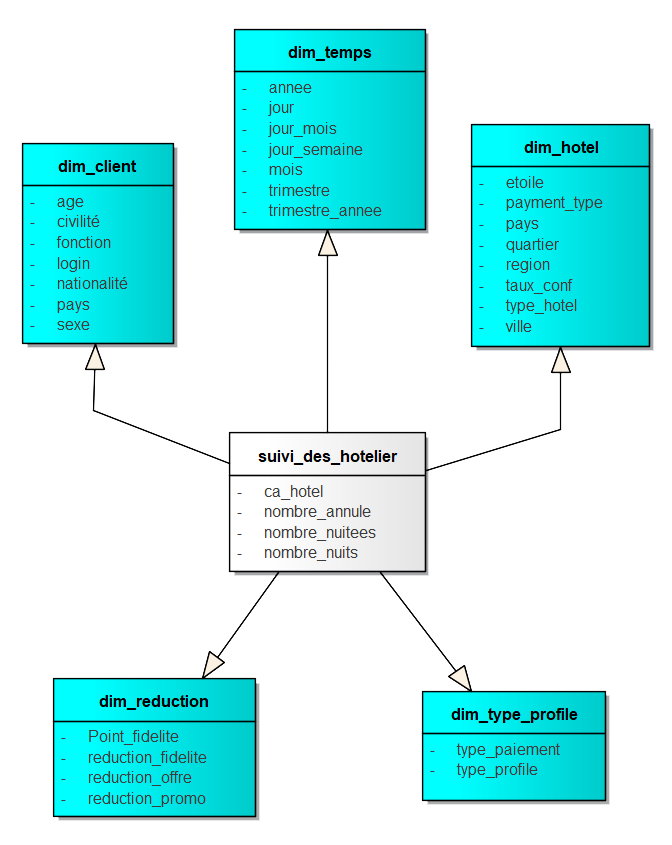
\includegraphics[scale=0.85]{images/cube_hotelier.png}
		\caption{Cube dimensionnel « Suivi des hoteliers ».}
		\label{use_bi_tools}
	\end{center}
\end{figure}

\begin{figure}[!htbp]
	\begin{center}
		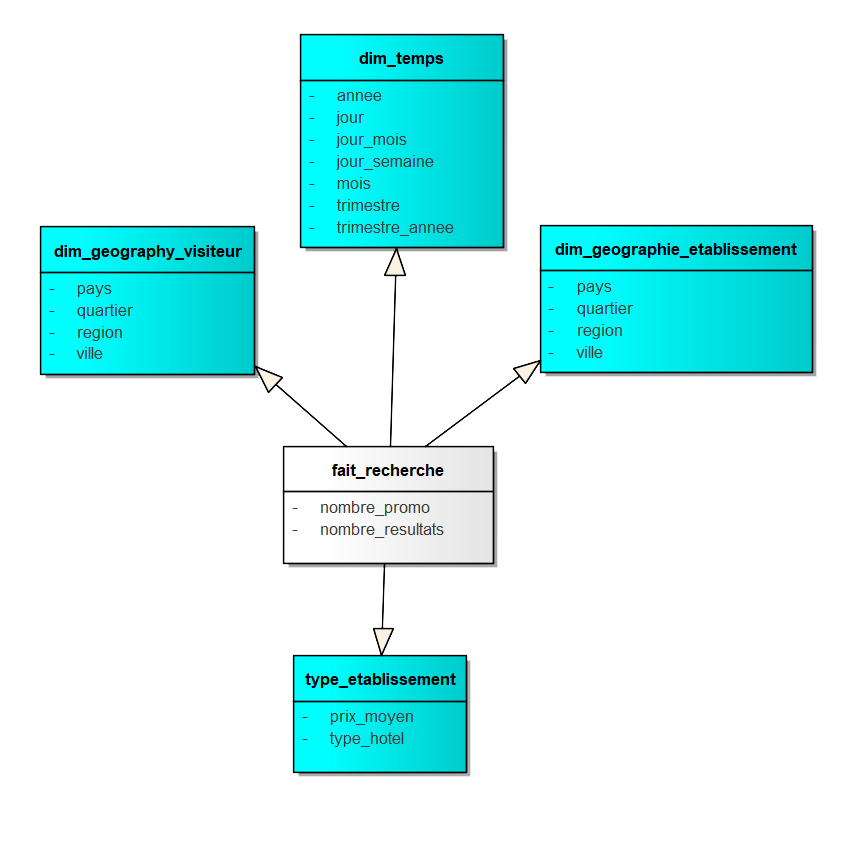
\includegraphics[scale=0.85]{images/cube_recherche.png}
		\caption{Cube dimensionnel « Recherche ».}
		\label{use_bi_tools}
	\end{center}
\end{figure}


\chapter{DÉPLOIEMENT}


Pour la réalisation et la mise en place de la solution, il a été nécessaire de recourir à un certain nombre d’outils et mettre en place des environnements d’exécution.
Ce chapitre a pour objectif, de décrire l’environnement mis en place et les outils utilisés, ainsi que de décrire l’environnement existant (matériels et logiciels), et dans lequel évoluera notre système.

\section{PARTIE WEB}
 Cette partie est celle qui sera accessible depuis la plateforme en ligne. Elle couvre les différents besoins exprimés pour les profils client, hôteliers et administrateurs. Elle sera réalisée sur le système de Hosteline. Ainsi, la finalité de cette mise en œuvre sera un système décisionnel qui fonctionne côte à côte avec le système opérationnel. Le diagramme de la figure qui suit est fait selon les formalismes du diagramme de déploiement spécifié plus haut. Il décrit le système mis en place pour cette partie.
 
\begin{figure}[!htbp]
	\begin{center}
		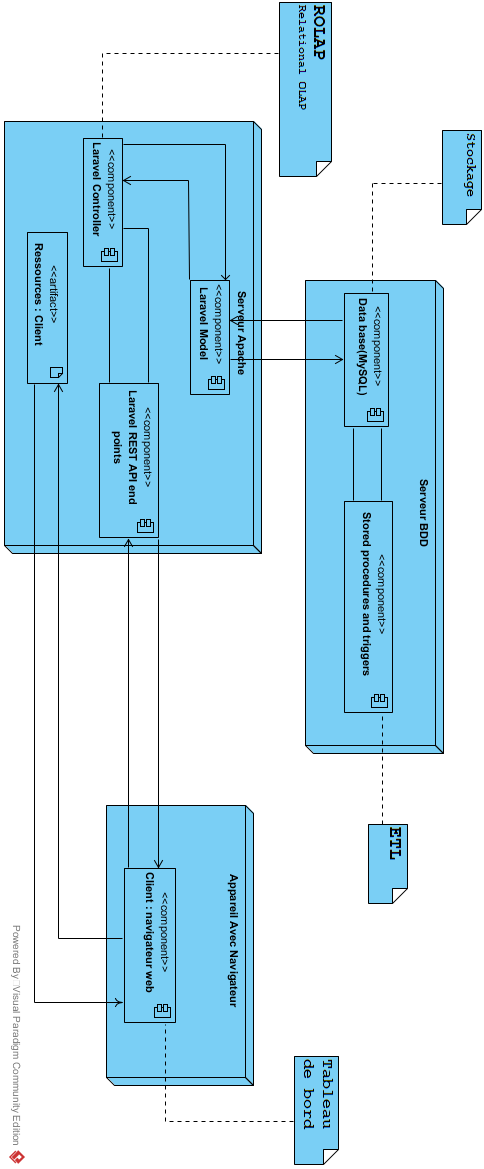
\includegraphics[scale=0.75]{images/deploy_web.png}
	\caption{Diagramme de déploiement de la partie web}
		\label{use_case_diagramme_one}
	\end{center}
\end{figure}

\cleardoublepage
\section{PARTIE DESKTOP}
Cette partie sera installé en local a l’entreprise sur une machine prévu a cette effet. C’est sur cette machine que sera installée la suite Pantaho. Le diagramme de la figure suivant explique comment ce système est mis en œuvre.

\begin{figure}[!htbp]
	\begin{center}
		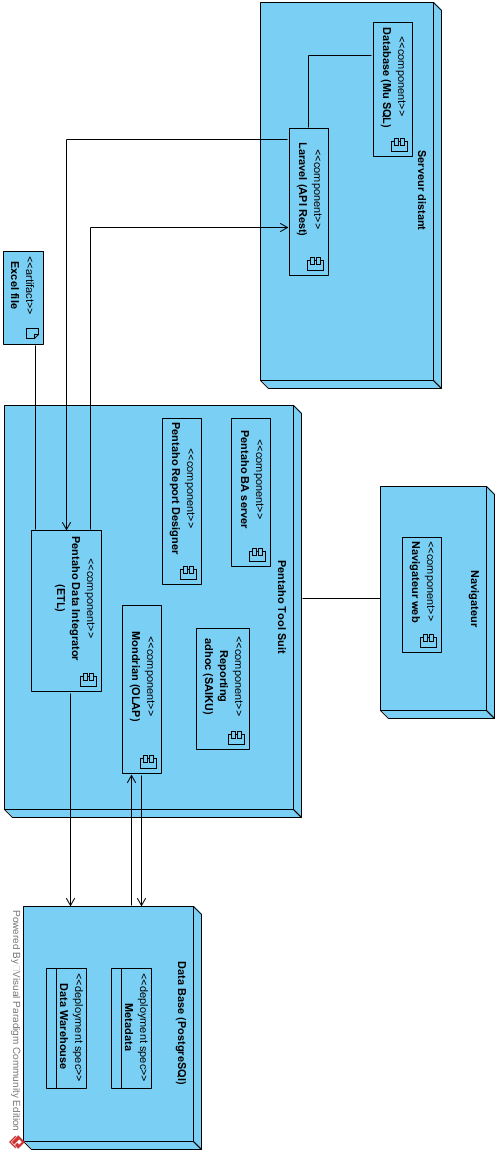
\includegraphics[scale=0.65]{images/deploy_desktop.png}
	\caption{Diagramme de déploiement de la partie desktop}
		\label{use_case_diagramme_one}
	\end{center}
\end{figure}






\chapter*{Conclusion}
\addcontentsline{toc}{chapter}{Conclusion}








%\backmatter
\pagestyle{back}
\renewcommand{\bibname}{Références} 

\begin{thebibliography}{9}
	
	\bibitem{ref14}[Kimball,1996], R. Kimball ; \emph{« Entrepôts de données : Guide pratique du concepteur de
Data Warehouse » };Wiley Computer Publishing 1996.
	
	
	\bibitem{ref15}[Kimball, 2002], R. Kimball et M. Ross ; \emph{« Entrepôts de Données : Guide Pratique de
Modélisation Dimensionnelle 2ème édition »}. Vuibert 2002.
	
	
	\bibitem{ref17} [Goglin, 1998] : J.F. Goglin;\emph{ « La Construction du Datawarehouse : du Datamart au
Dataweb »} ; Hermes 1998.
	
	\bibitem{ref17} [Le Moigne, 1977] : Le Moigne J.L., \emph{« La théorie du système général, théorie de la
modélisation »} , P.U.F., 1977.
	
	 \bibitem{ref18} [Rainardi 2008]  : Vincent Rainardi, \emph{« Building a Data Warehouse: With Examples in SQL Server »} ; 
	 
	 \bibitem{ref19} Alex Meadows : \emph{« Pentaho Data Integration Cookbook Second Edition »} ; 2013 Packt Publishing
	 
	 \bibitem{ref20} Joel Latino, Harris Ward : \emph{« Pentaho Analytics for MongoDB Cookbook »} ; 2015 Packt Publishing 
	
	 \bibitem{ref21} Pantaho Corporate : \emph{« Introducing the Pentaho BI Suite Community Edition »}
	 
	 \bibitem{ref22} Hitachi Vantara : https://help.pentaho.com/Documentation/8.1
	 
	 \bibitem{ref24} Dr TSOPZE N. : Système d'information décisionnels, année académique 2016 - 2017
	 
	 \bibitem{ref25} Dr TOTO Philippe : Business intelligence, année académique 2017 - 2018
	  
	
\end{thebibliography}

\addcontentsline{toc}{chapter}{Références}






\appendix
\chapter{titre annexe}

\section{titre 1}














\renewcommand{\contentsname}{Table des matières} 
\setcounter{tocdepth}{3}
\tableofcontents
\addcontentsline{toc}{chapter}{Table des matières}





\end{document}